\documentclass[10pt]{beamer}

\usetheme[progressbar=frametitle]{metropolis}
\usepackage{appendixnumberbeamer}

\usepackage{booktabs}
\usepackage[scale=2]{ccicons}

\usepackage{pgfplots}
\usepgfplotslibrary{dateplot}

\usepackage{xspace}
\newcommand{\themename}{\textbf{\textsc{metropolis}}\xspace}

% \definecolor{mDarkBrown}{HTML}{604c38}
\definecolor{mDarkTeal}{HTML}{333333}
\definecolor{mLightBrown}{HTML}{ec5a2c}
% \definecolor{mLightGreen}{HTML}{14B03D}
\definecolor{dockerBlue}{HTML}{0972aa}

\setbeamercolor{frametitle}{bg=dockerBlue}

\usepackage{biblatex}
\usepackage{filecontents}
\usepackage{xpatch}
\addbibresource{../paper.bib}
\setbeamertemplate{bibliography item}{}

\title{Docker}
% \subtitle{}
% \date{\today}
\date{}
\author{Julian Tiemann}
\institute{Universität Hamburg}
% \titlegraphic{\hfill\includegraphics[height=1.5cm]{logo.pdf}}

\begin{document}

\maketitle

\begin{frame}{Table of contents}
  \setbeamertemplate{section in toc}[sections numbered]
  \tableofcontents[hideallsubsections]
\end{frame}

\section{Einleitung}

\begin{frame}[fragile]{Einleitung}

  Einleitung

\end{frame}

\section{Virtuelle Machinen}

\begin{frame}[fragile]{Virtual Machine}
  \begin{columns}[T,onlytextwidth]
    \column{0.33\textwidth}
      \begin{itemize}
        \item Bla Bla Bla 1
        \item Bla Bla Bla 2
        \item Bla Bla Bla 3
      \end{itemize}
    \column{0.66\textwidth}
      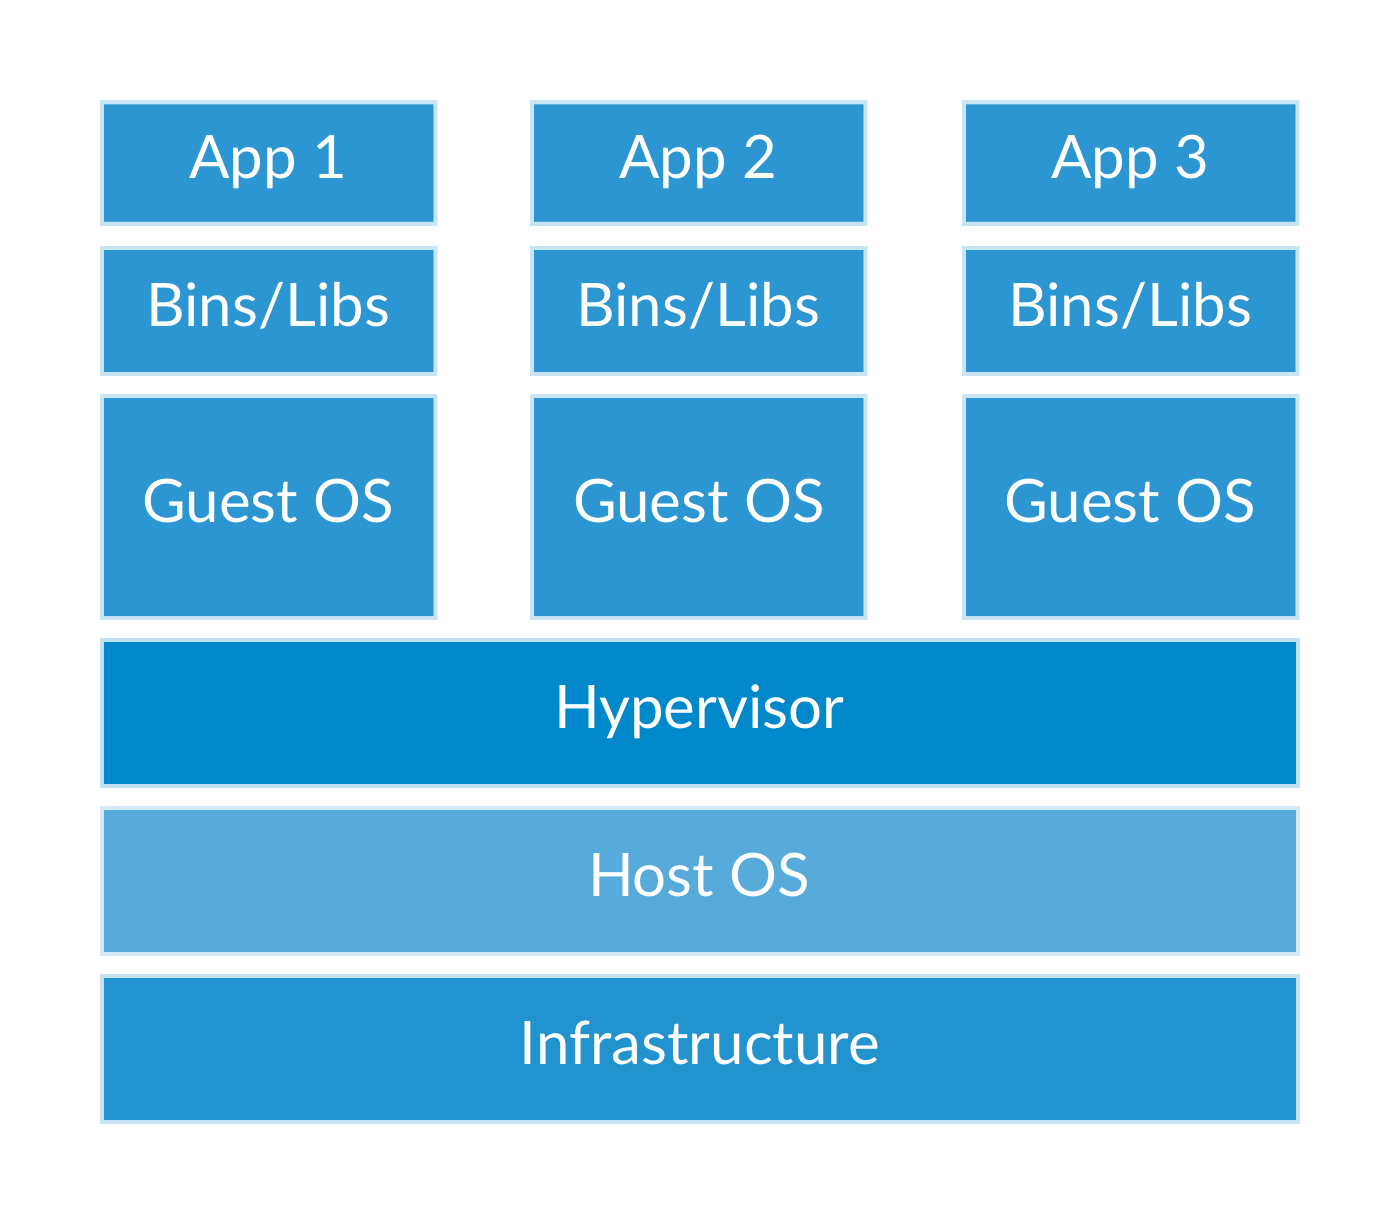
\includegraphics[width=1\textwidth]{../images/1-docker-vm.png}
  \end{columns}
\end{frame}

\begin{frame}{Hypervisors}
  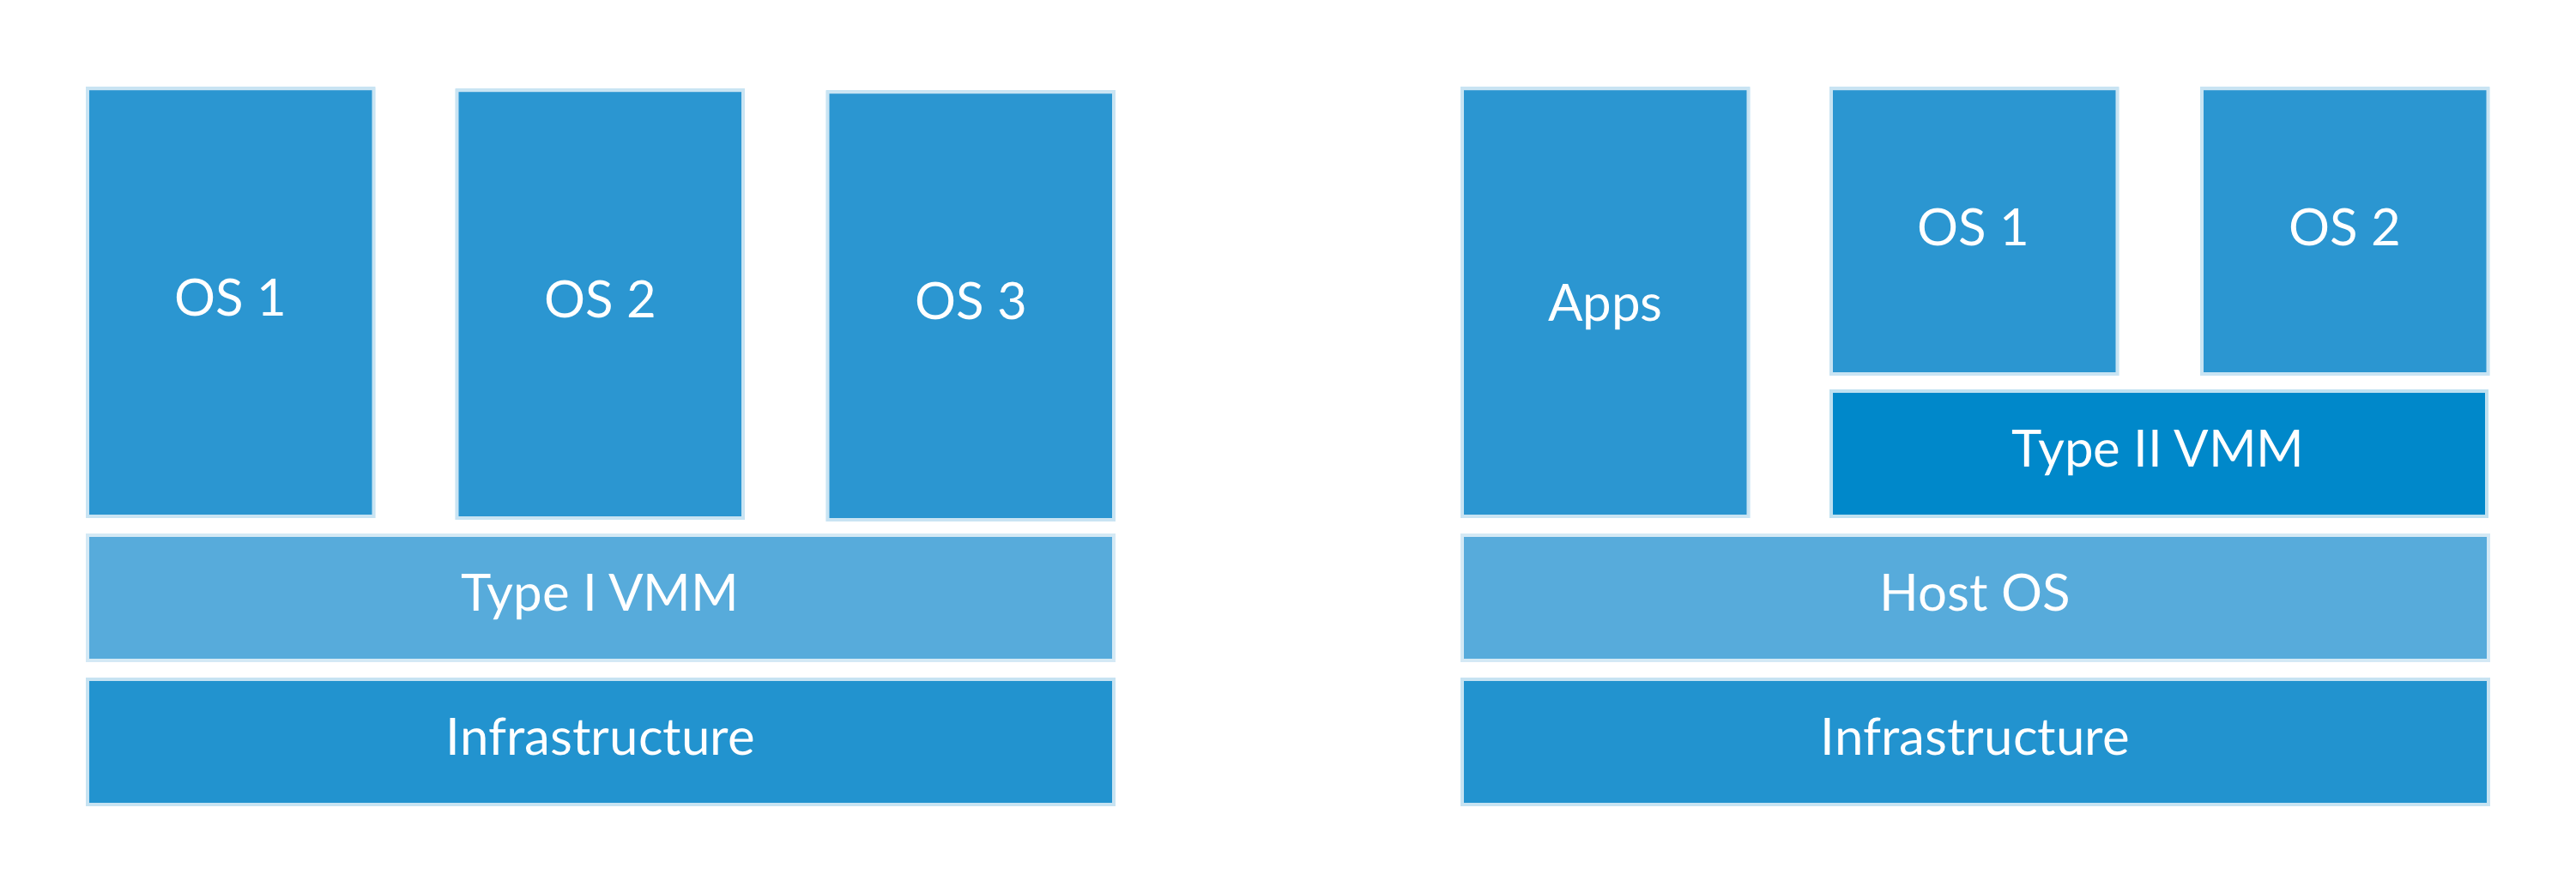
\includegraphics[width=1\textwidth]{../images/2-hypervisors.png}
\end{frame}

\section{Container}

\begin{frame}{Container Typen}
  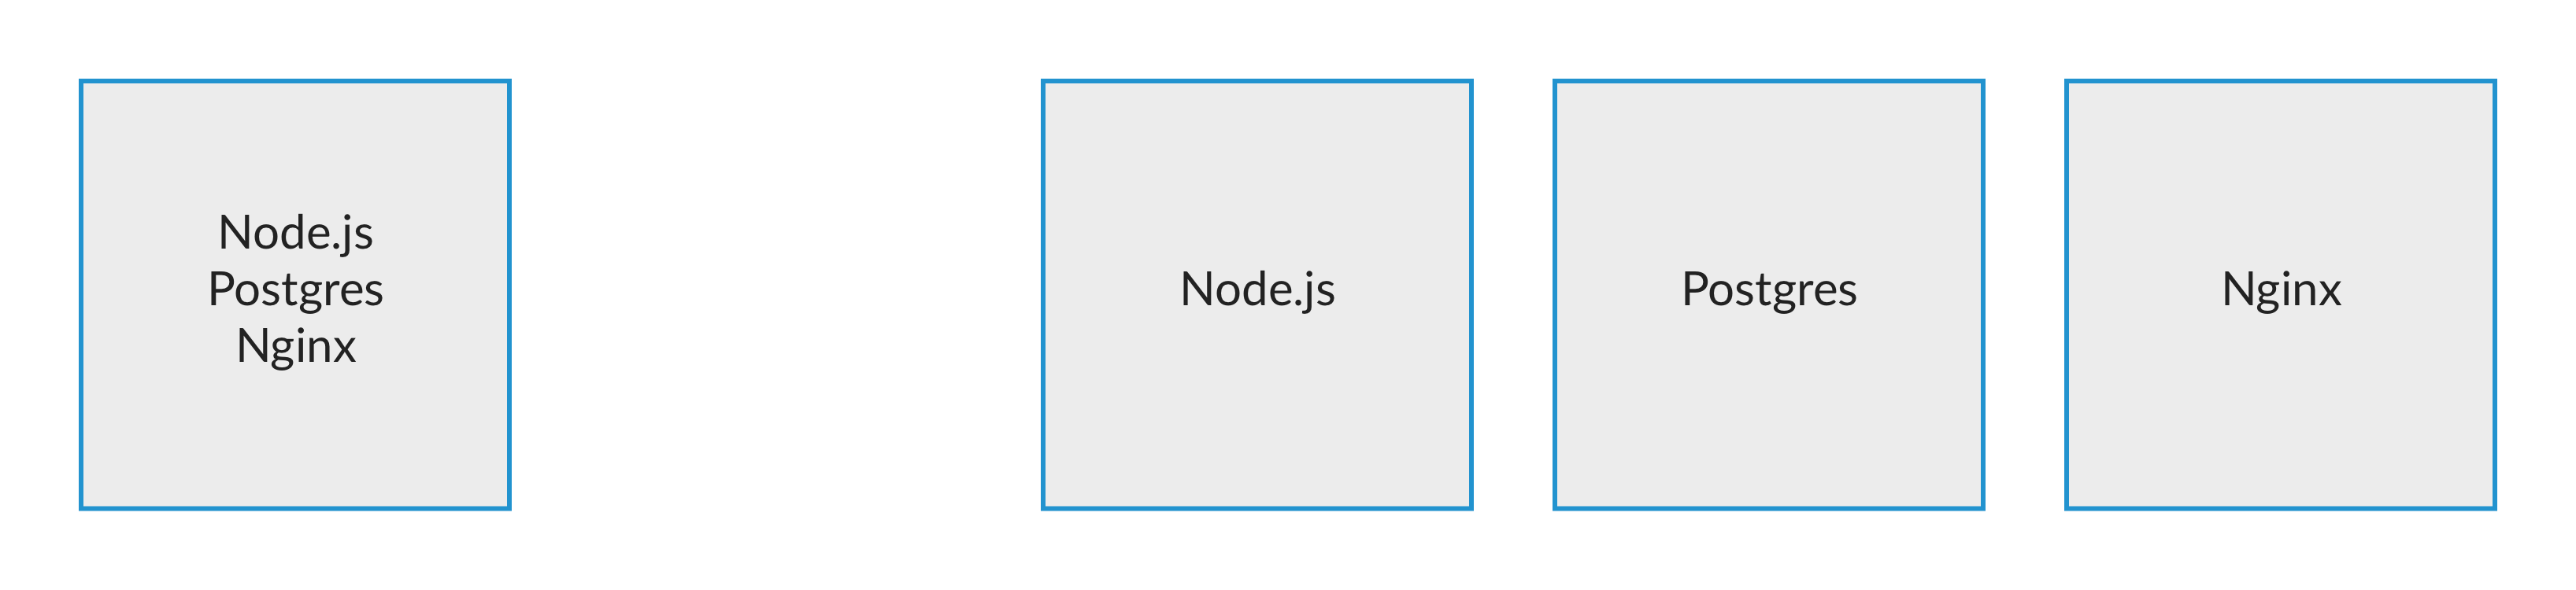
\includegraphics[width=1\textwidth]{../images/4-os-specialized-containers.png}
  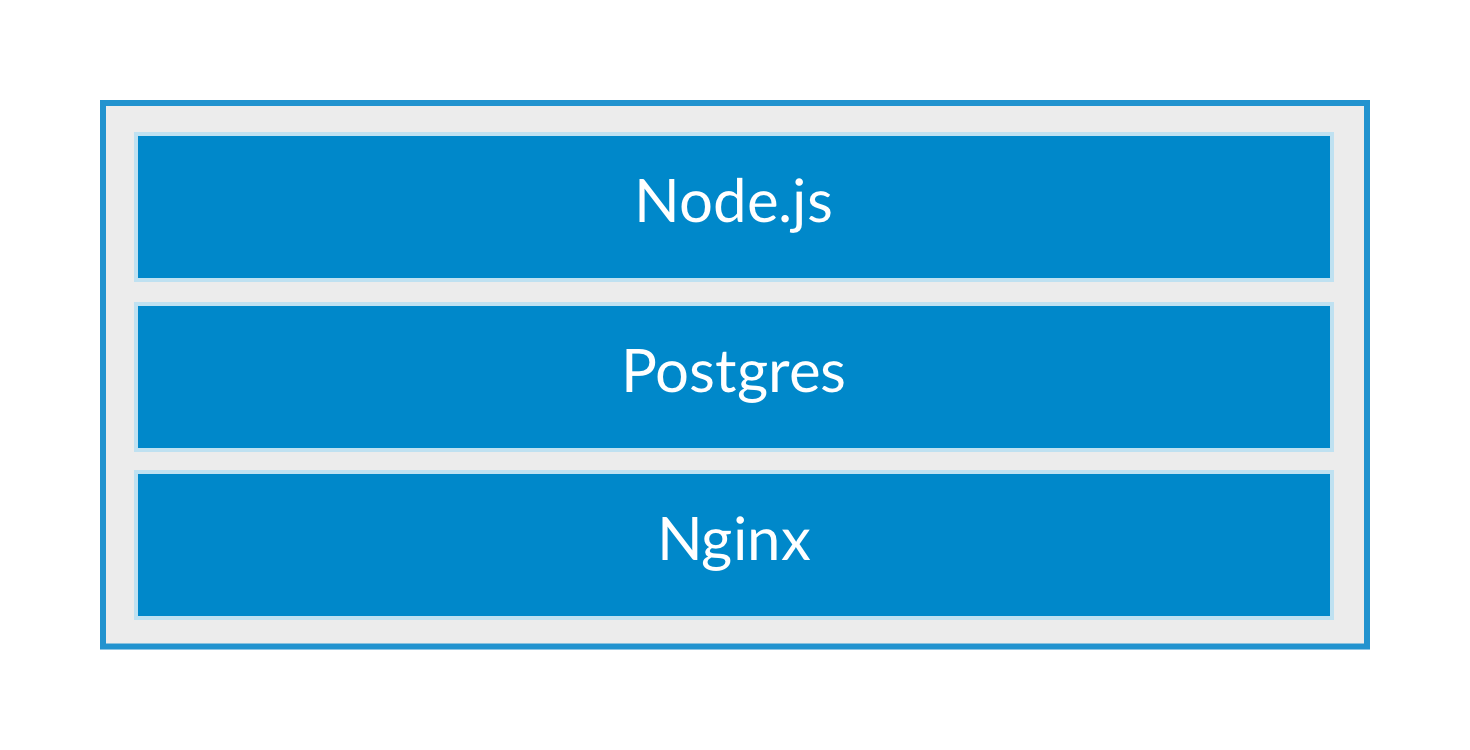
\includegraphics[width=1\textwidth]{../images/5-application-container.png}
\end{frame}

\begin{frame}{Container vs VM}
  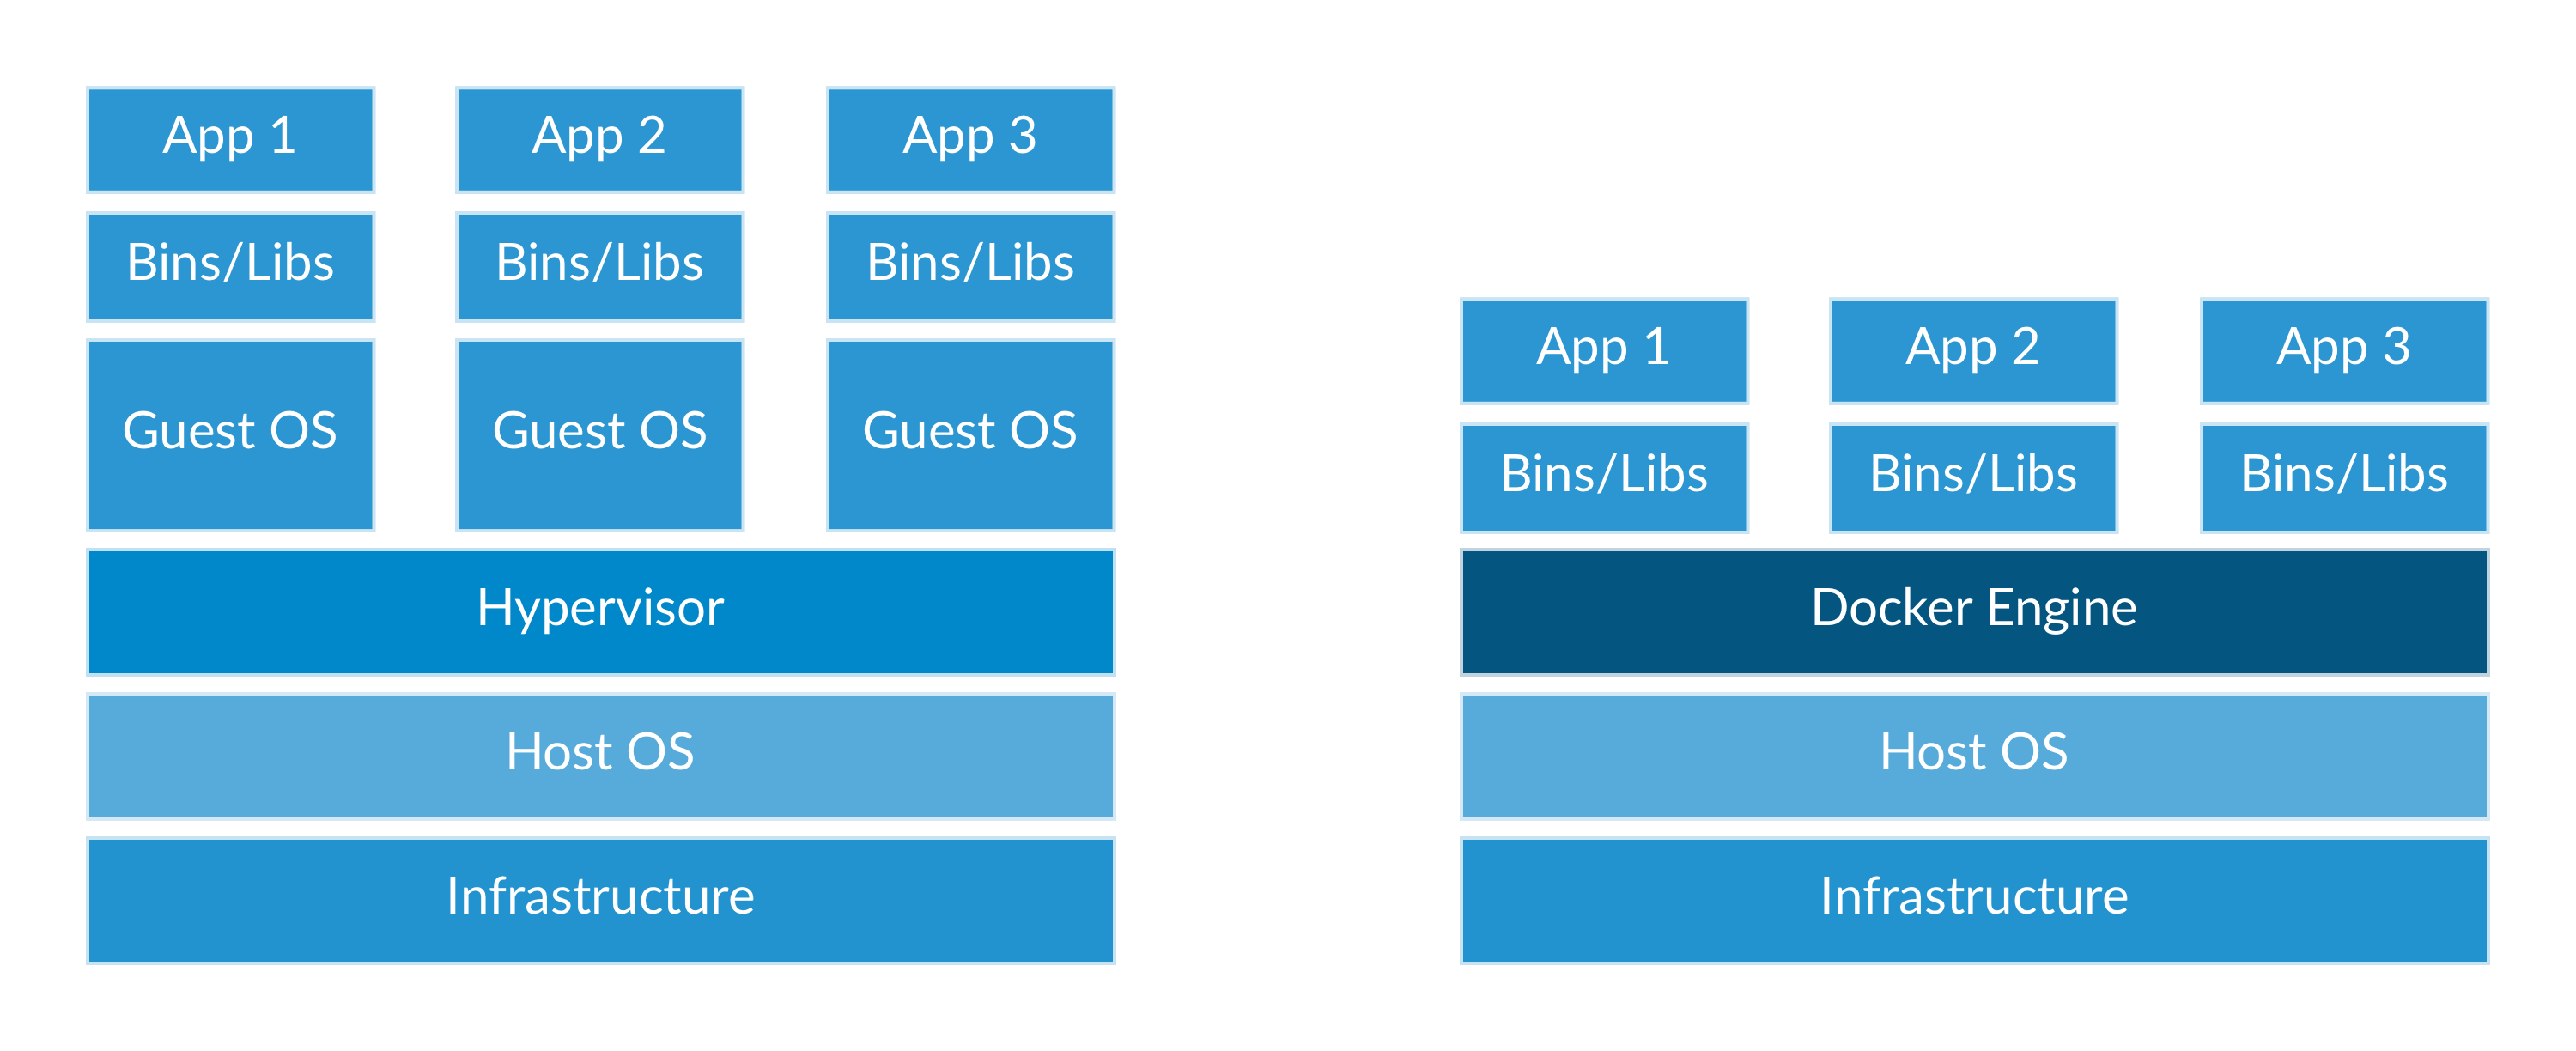
\includegraphics[width=1\textwidth]{../images/6-container-vm.png}
\end{frame}

\begin{frame}{Container und VMs kombiniert}
  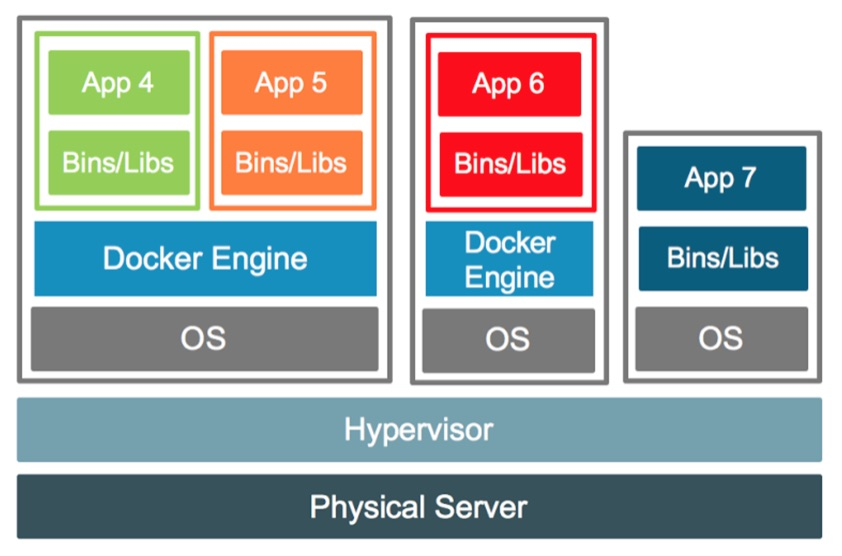
\includegraphics[width=1\textwidth]{../images/7-container-vm-combined.jpg}
\end{frame}

\section{Docker}

\begin{frame}{Docker Engine}
  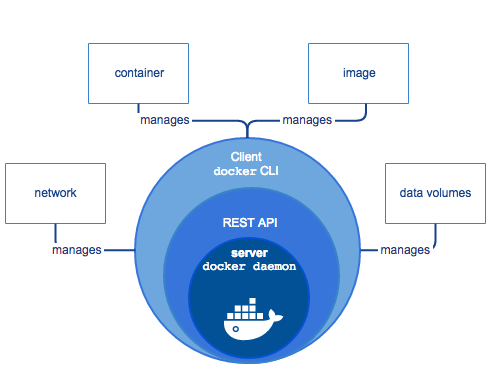
\includegraphics[width=1\textwidth]{../images/8-docker-engine.png}
\end{frame}

\begin{frame}{Docker Images}
  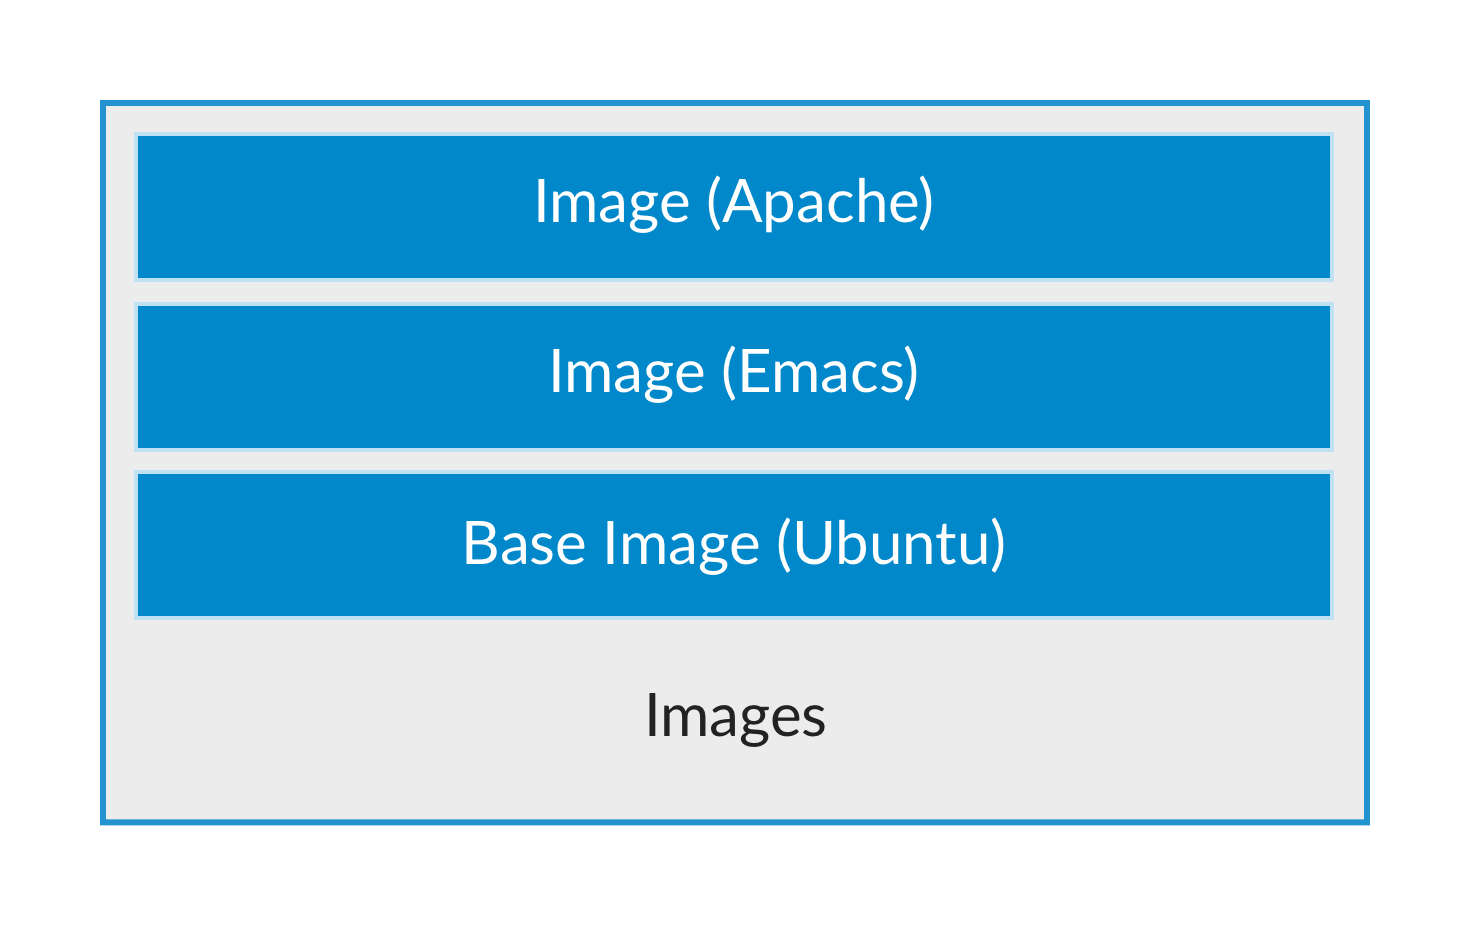
\includegraphics[width=1\textwidth]{../images/9-docker-image.png}
\end{frame}

\begin{frame}{Docker Image Layer Sharing}
  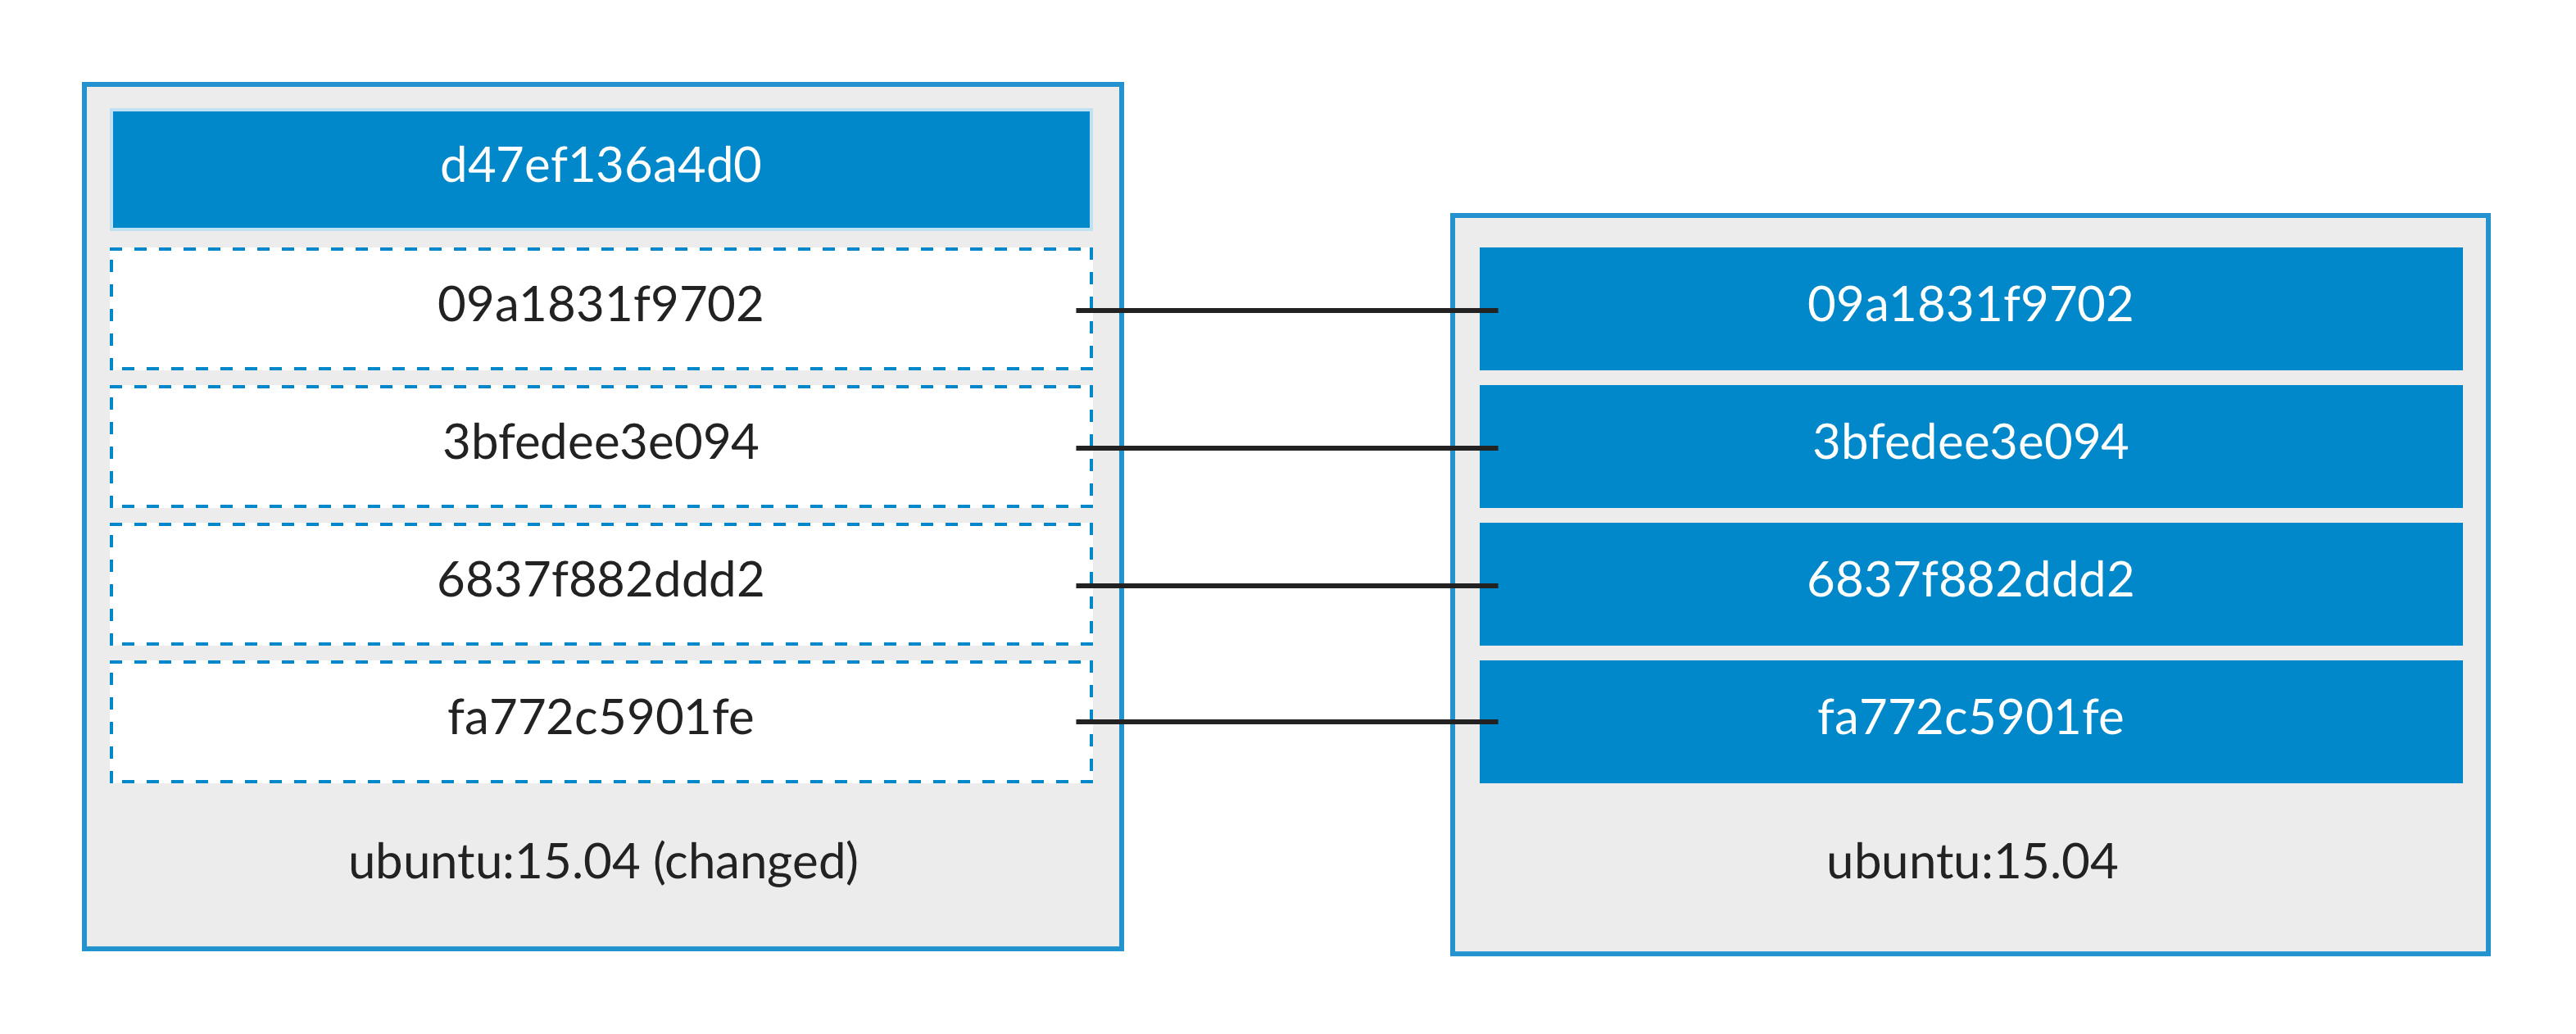
\includegraphics[width=1\textwidth]{../images/10-docker-image-layer-sharing.png}
\end{frame}

\begin{frame}{Docker Container}
  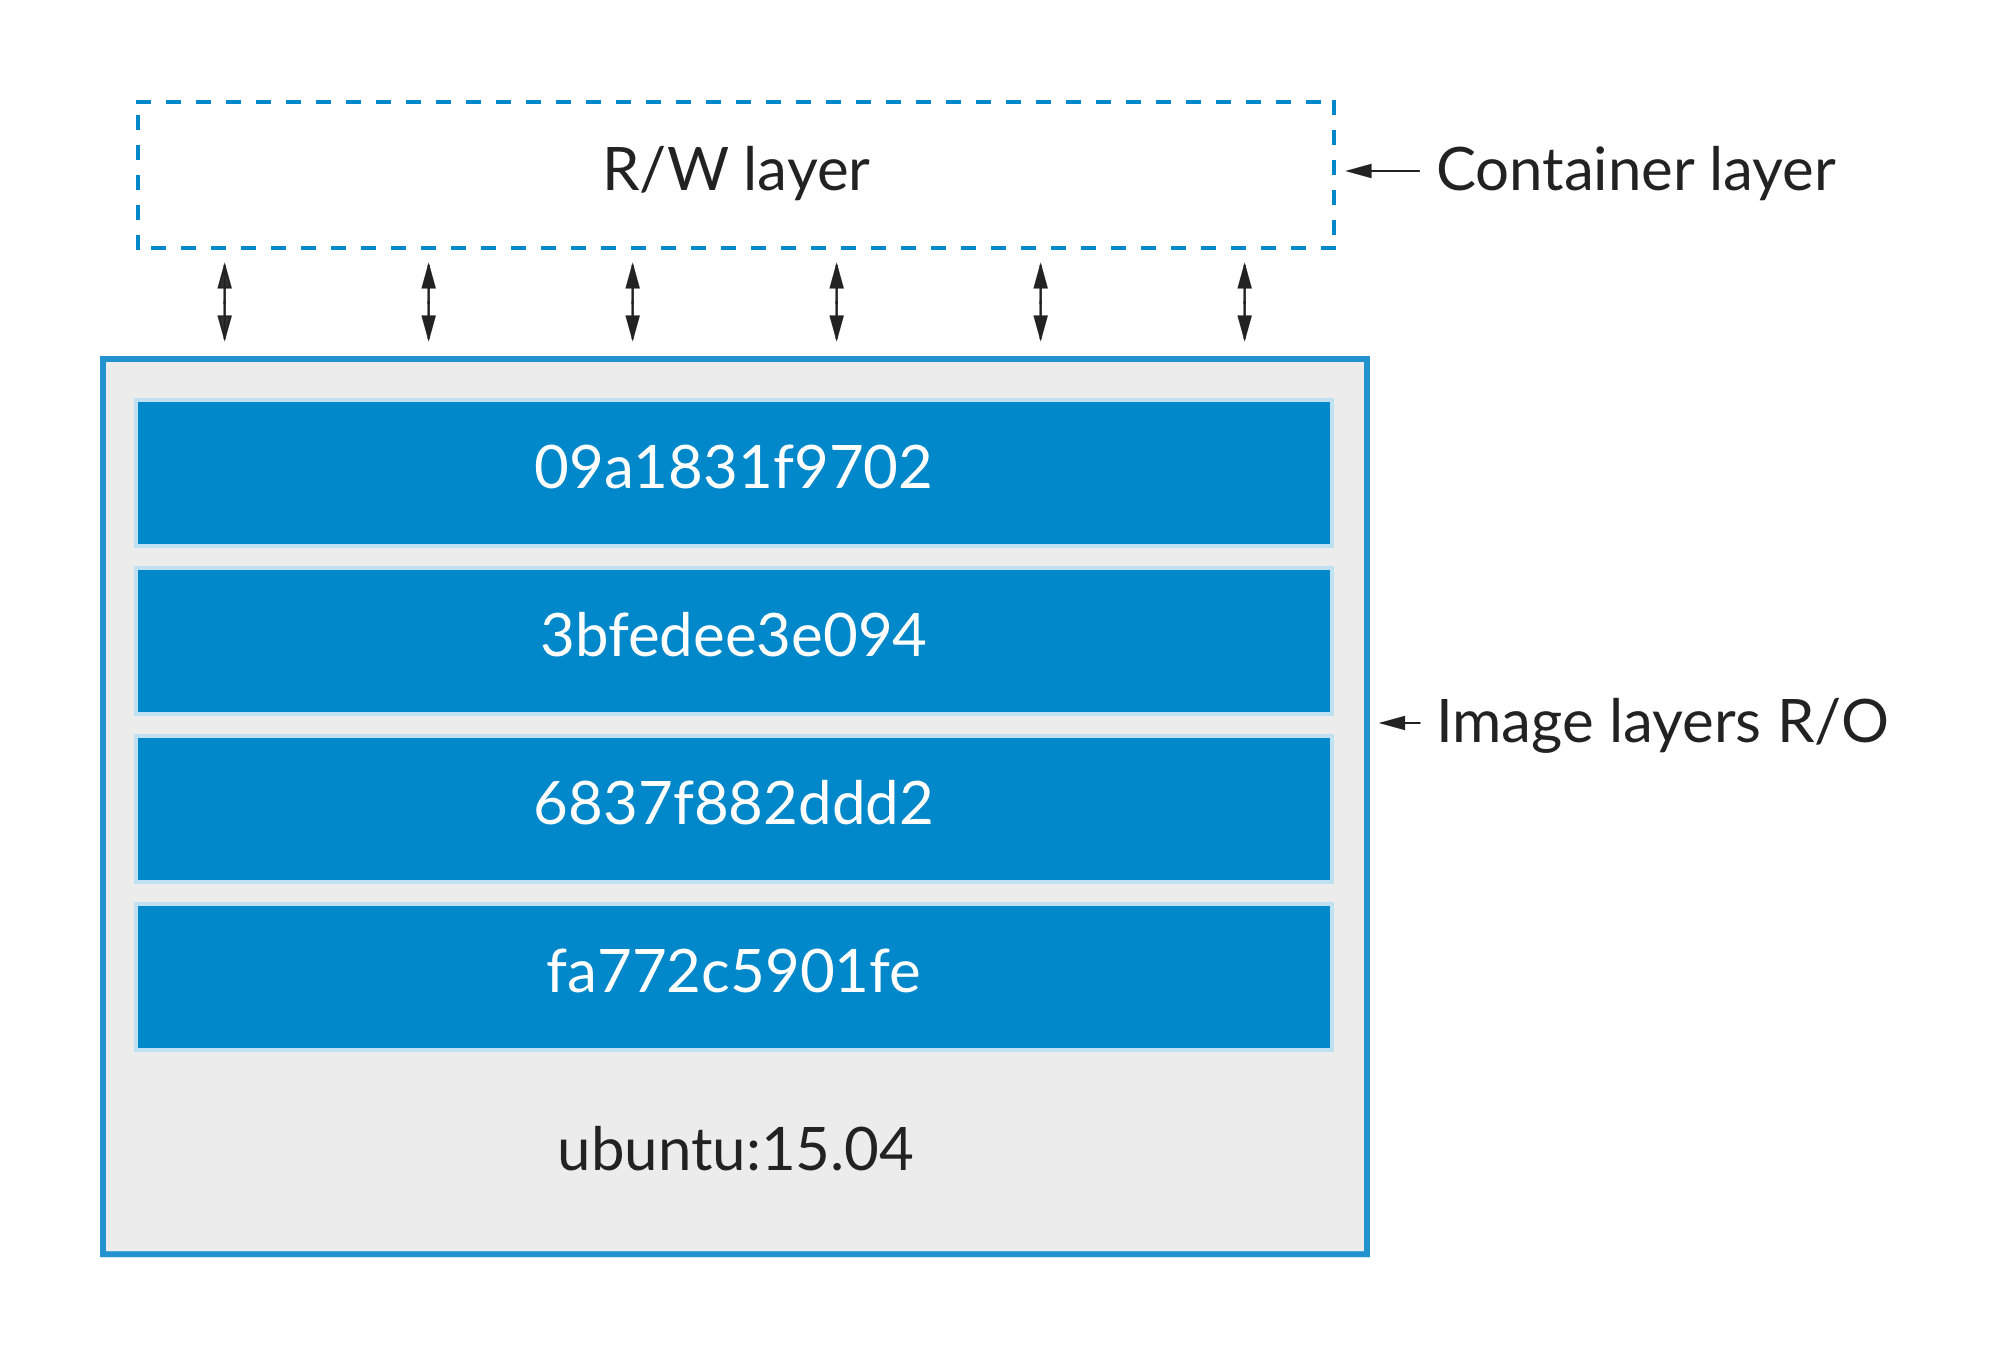
\includegraphics[width=1\textwidth]{../images/11-docker-container.png}
\end{frame}

\begin{frame}{Docker Daemon}
  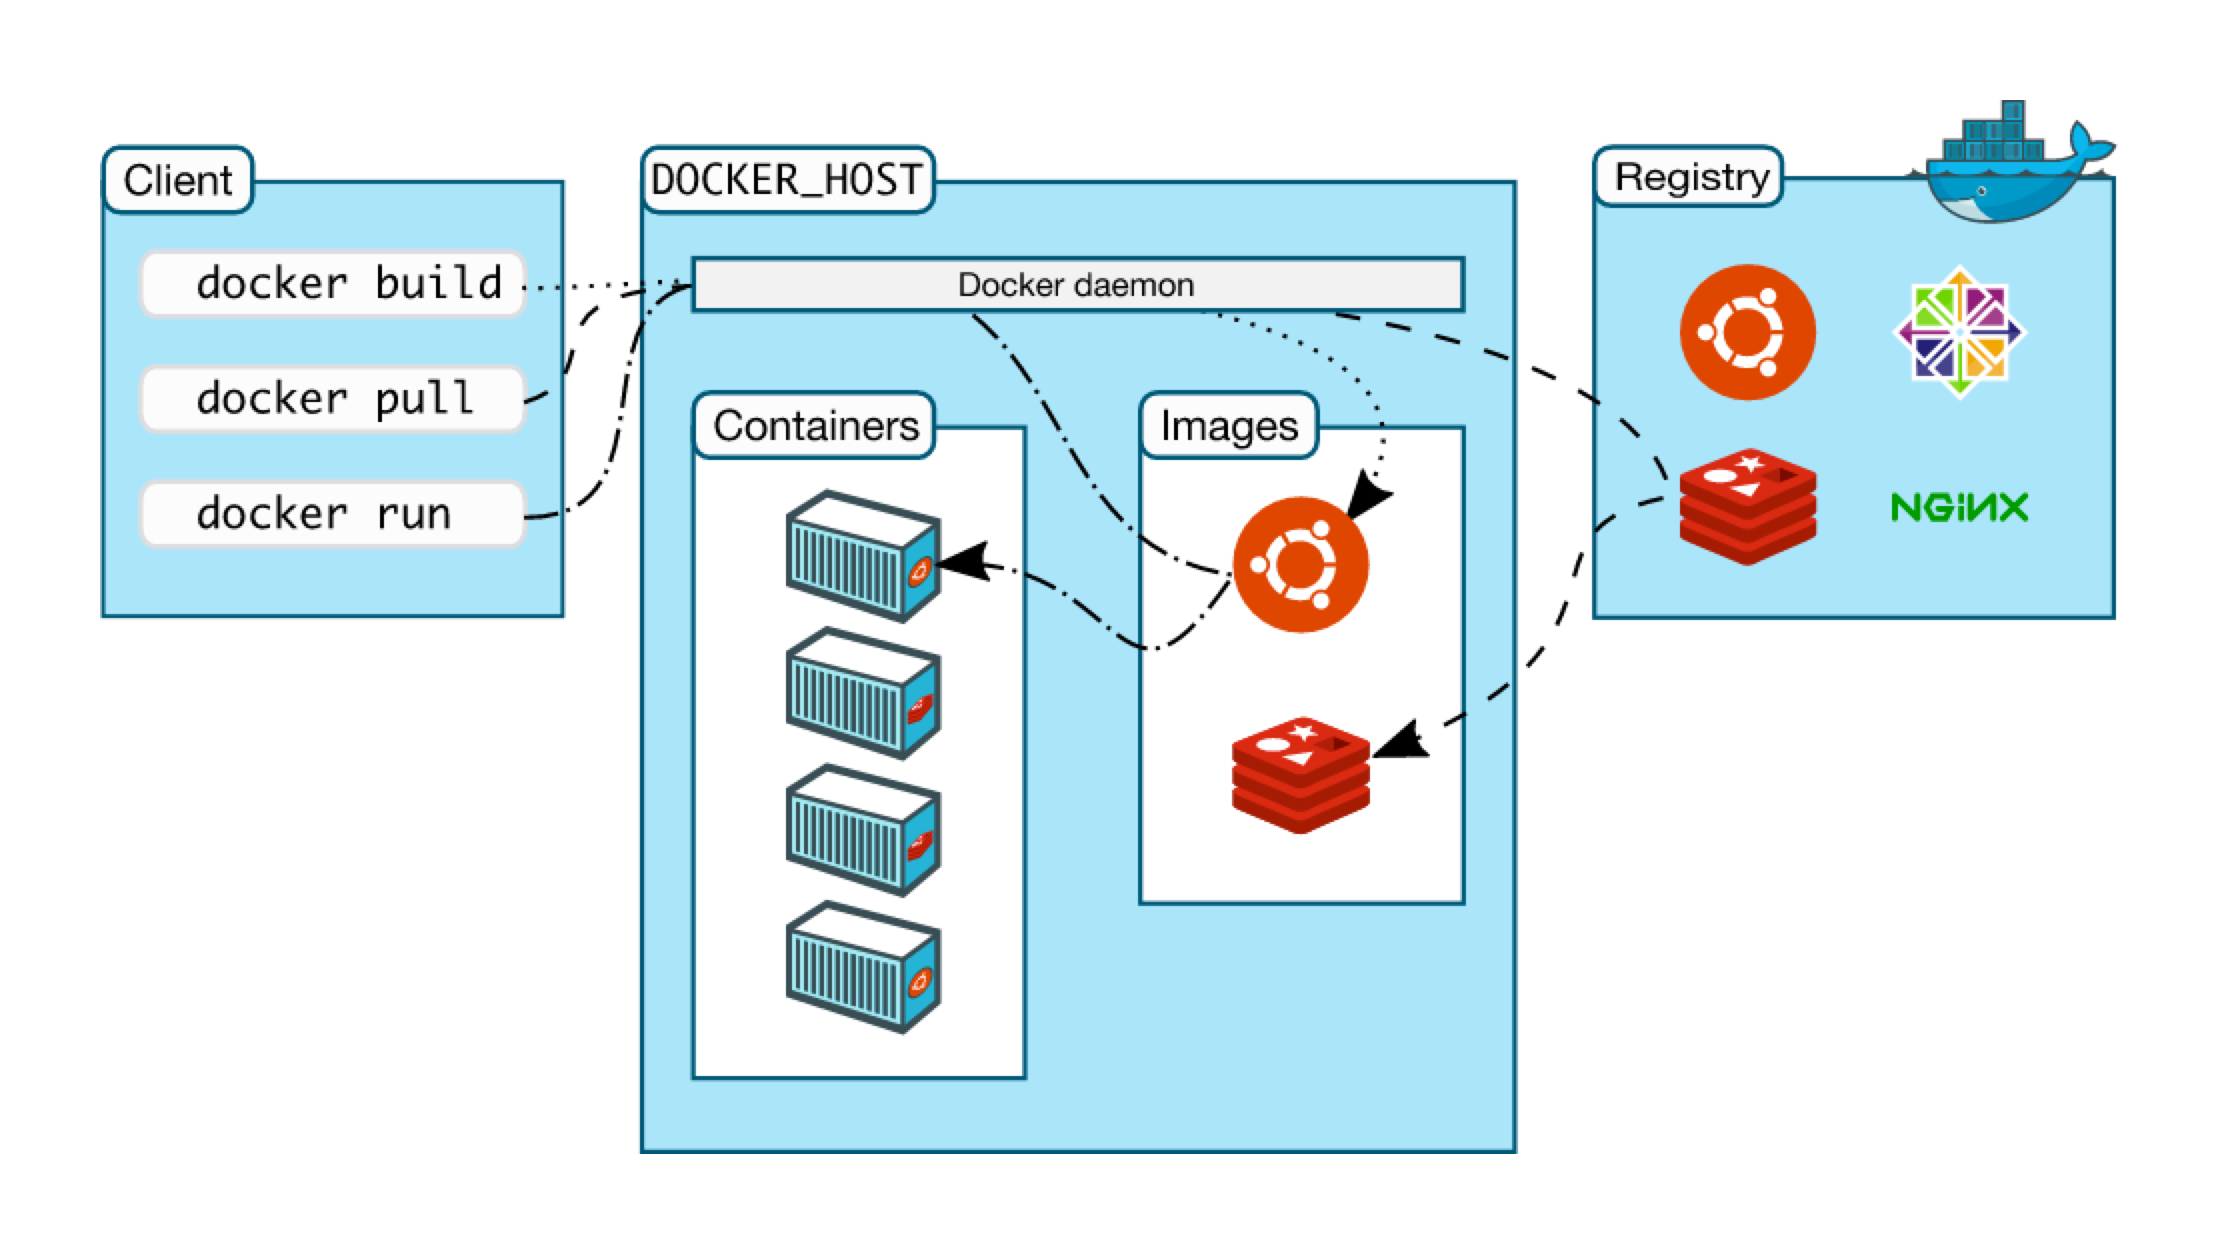
\includegraphics[width=1\textwidth]{../images/12-docker-daemon.png}
\end{frame}

\section{Fazit}

\begin{frame}{Fragen}

  Fragen?
  
\includegraphics[width=1\textwidth]{../images/14-docker-swarm-hero2.png}

\end{frame}

\appendix

\begin{frame}[allowframebreaks]{References}

  % \bibliography{../paper.bib}
  % \bibliographystyle{abbrv}
  \printbibliography

\end{frame}

\end{document}
